\begin{exercise}
	Ο πίνακας ορίζει ένα μετασχηματισμό που ονομάζεται Shearing. Για $b = 0$, έχουμε shearing στην κατεύθυνση $x$ ενώ για $a=0$ έχουμε shearing στην κατεύθυνση $y$. Με τη βοήθεια αυτού, να βρεθεί ο μετασχηματισμός $M$ που μετατρέπει τον ρόμβο με κορυφές $A (0, \sqrt{2}), B(\sqrt{2},0), \Gamma (0, -\sqrt{2}, \Delta(-\sqrt{2},0)$ στο παραλληλόγραμμο με κορυφές $A^{'} (0,1), B^{'} (1,1), \Gamma^{'}(0,-1), \Delta^{'}$ όπως φαίνεται παρακάτω.

\begin{figure}[h!]
	\begin{center}
		\begin{minipage}[b]{0.4\textwidth} % Top-left image
		    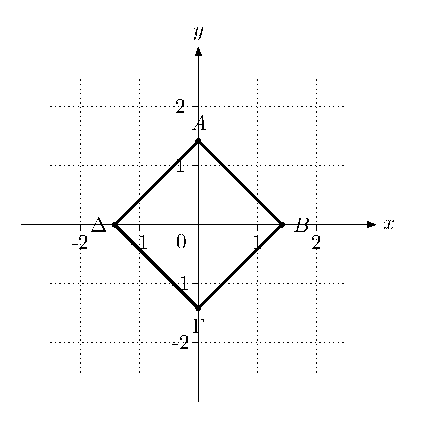
\includegraphics[width=\textwidth]{Chapter2/Exercises/ex2-graph1.pdf}
		\end{minipage}%
	\hfill
		\begin{minipage}[b]{0.4\textwidth} % Top-right image
		    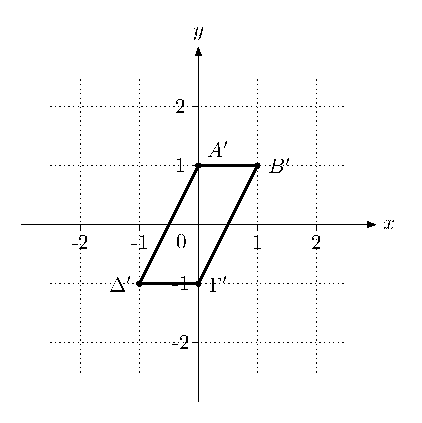
\includegraphics[width=\textwidth]{Chapter2/Exercises/ex2-graph2.pdf}
		\end{minipage}
	\end{center}
%\caption{.}
\end{figure}	
	
\end{exercise}


\begin{solution}

\textbf{\underline{1ος τρόπος}}: 

\begin{enumerate}
	  \item Scaling κατά $S_x = S_y = \cfrac{1}{\sqrt{2}}$ (Πολλαπλασιασμός με πίνακα $S_{S_x, S_y}$)
	  \item Shearing στο $y$ με $b=1$ (Πολλαπλασιασμός με πίνακα $Sh_y$)
\end{enumerate}

\[
	M = 
		\begin{bmatrix}
			1 & 0 \\
			1 & 1
		\end{bmatrix}
	\cdot
		\begin{bmatrix}
			\cfrac{1}{\sqrt{2}} & 0 \\
			0 & \cfrac{1}{\sqrt{2}}
		\end{bmatrix}
	=	
		\begin{bmatrix}
			\cfrac{1}{\sqrt{2}} & 0 \\
			 \cfrac{1}{\sqrt{2}} & \cfrac{1}{\sqrt{2}}
		\end{bmatrix}
	=
	\begin{bmatrix}
			\cfrac{\sqrt{2}}{2} & 0 \\
			 \cfrac{\sqrt{2}}{2} & \cfrac{\sqrt{2}}{2}
		\end{bmatrix}	
\]

Για να υπολογίσουμε πώς ο παραπάνω μετασχηματισμός επιδράσει στο σχήμα: 
\[
	A (0, \sqrt{2}), B(\sqrt{2},0), \Gamma (0, -\sqrt{2}, \Delta(-\sqrt{2},0),
\]	
θα πολλαπλασιάσουμε τον πίνακα τον συντεταγμένων του σχήματος με τον πίνακα του μετασχηματισμού.

\[
M \cdot V = 
	\begin{bmatrix}
		\frac{1}{\sqrt{2}} & 0 \\
		\frac{1}{\sqrt{2}} & \frac{1}{\sqrt{2}} 
	\end{bmatrix}
\cdot 
	\begin{bmatrix}
		0 & \sqrt{2} & 0 & -\sqrt{2} \\
		\sqrt{2} & 0 & -\sqrt{2} & 0 
	\end{bmatrix}
	=
	\begin{bmatrix}
		0 & 1 & 0 & -1 \\
		1 & 1 & -1 & -1
	\end{bmatrix}	
\]


\textbf{\underline{2ος τρόπος}}: 

\begin{enumerate}
	  \item Στροφή κατά γωνία $45^\circ$ (Πολλαπλασιασμός με πίνακα $R_{45^\circ}$)
	  \item Scaling $S_x = \cfrac{1}{2}, S_y  = 1$ (Πολλαπλασιασμός με πίνακα $S_{S_x, S_y}$)
	  \item Shearing $S_{h_x}, a = \cfrac{1}{2}, b=0$ (Πολλαπλασιασμός με πίνακα $S_{h_x}$) 
\end{enumerate}

Για να υπολογίσουμε πώς ο παραπάνω μετασχηματισμός επιδράσει στο σχήμα $A (0, \sqrt{2}), B(\sqrt{2},0), \Gamma (0, -\sqrt{2}, \Delta(-\sqrt{2},0)$, θα πολλαπλασιάσουμε τον πίνακα τον συντεταγμένων του σχήματος με τον πίνακα του μετασχηματισμού, δηλαδή με τον πίνακα:

\[
	M = S_{h_x} \cdot S_{S_x, S_y} \cdot R_{\theta}  = 
	\begin{bmatrix}
		1 & \frac{1}{\sqrt{2}} \\
		0 & 1 
	\end{bmatrix}
\cdot 
	\begin{bmatrix}
		\frac{1}{\sqrt{2}} & 0 \\
		0 & 1
	\end{bmatrix}
\cdot
	\begin{bmatrix}
		\cfrac{\sqrt{2}}{2} & -\cfrac{\sqrt{2}}{2} \\
			 \cfrac{\sqrt{2}}{2} & \cfrac{\sqrt{2}}{2}
	\end{bmatrix}	
	=
	\begin{bmatrix}
		\cfrac{\sqrt{2}}{2} & 0 \\
			 \cfrac{\sqrt{2}}{2} & \cfrac{\sqrt{2}}{2}
	\end{bmatrix}
\] 

\end{solution}